\section{Motivations}
\begin{frame}{Motivations}
  \begin{figure}
    \center
    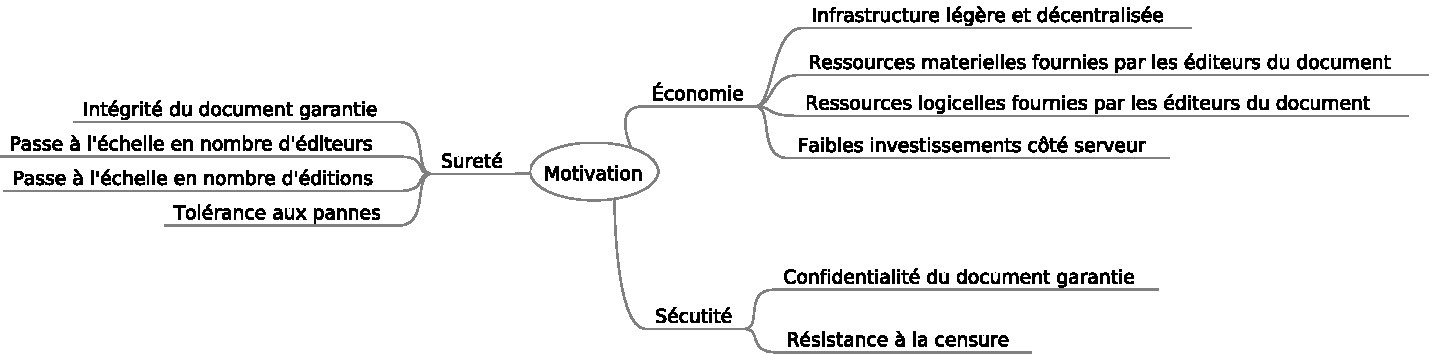
\includegraphics[width=\textwidth]{includes/motivations.pdf}
    \caption{Motivations -- carte heuristique}
  \end{figure}
\end{frame}
% Voilà ce qu'il en est des motivation économiques, techniques et sociales; mais
% à côté de ça, il y a une autre motivations, c'est que ce projet est également
% une vitrine pour les idées de la recherches puisqu'il utilise à la fois
% l'algorithme du logoot (dire pq) et le langage ciojo (dire pq) qui sont tous
% les deux issues du monde de la recherche. Et donc pour les équipes de
% recherches en charge de ces deux technologies, ce projet peut-être vue comme
% un prototype. Et du coup, se projet à susciter l'interressement à la fois de
% m P. Molli, en charge de l'équie GDD du Lina et initiateur de l'algortihme
% logoot ainsi que monsieur M.Sudholt en charge de l'équipe ASCOLA et du langage
% CRIOJO.
\begin{frame}{Motivations}
  \begin{itemize}
    \item Le projet est une vitrine pour les idées de la Recherche.
    \item Le projet est un prototype pour les technologies \textbf{Logoot},
    \textbf{Criojo} et des outils de l'ingénierie des modèles.
    \item Le projet suscite l'intérêt des équipes Inria \textbf{GDD},
    \textbf{ASCOLA} et \textbf{AtlanMod} et permettrait d'initier des
    collaborations entre les équipes.
  \end{itemize}
\end{frame}

